\chapter{Astrophysics around neutrons stars}
\chapterimage[width=15cm]{wordcloud/chap3b.png}


Let us try and estimate the energetics of different phenomena of what we can observe from neutron stars.\mnote{Energy output}
Few possible stable sources of energy exists: thermal, gravitational, rotational, and magnetic.
In addition, unstable fusion processes can also power some observable phenomena.




\begin{figure}[t]
\centering
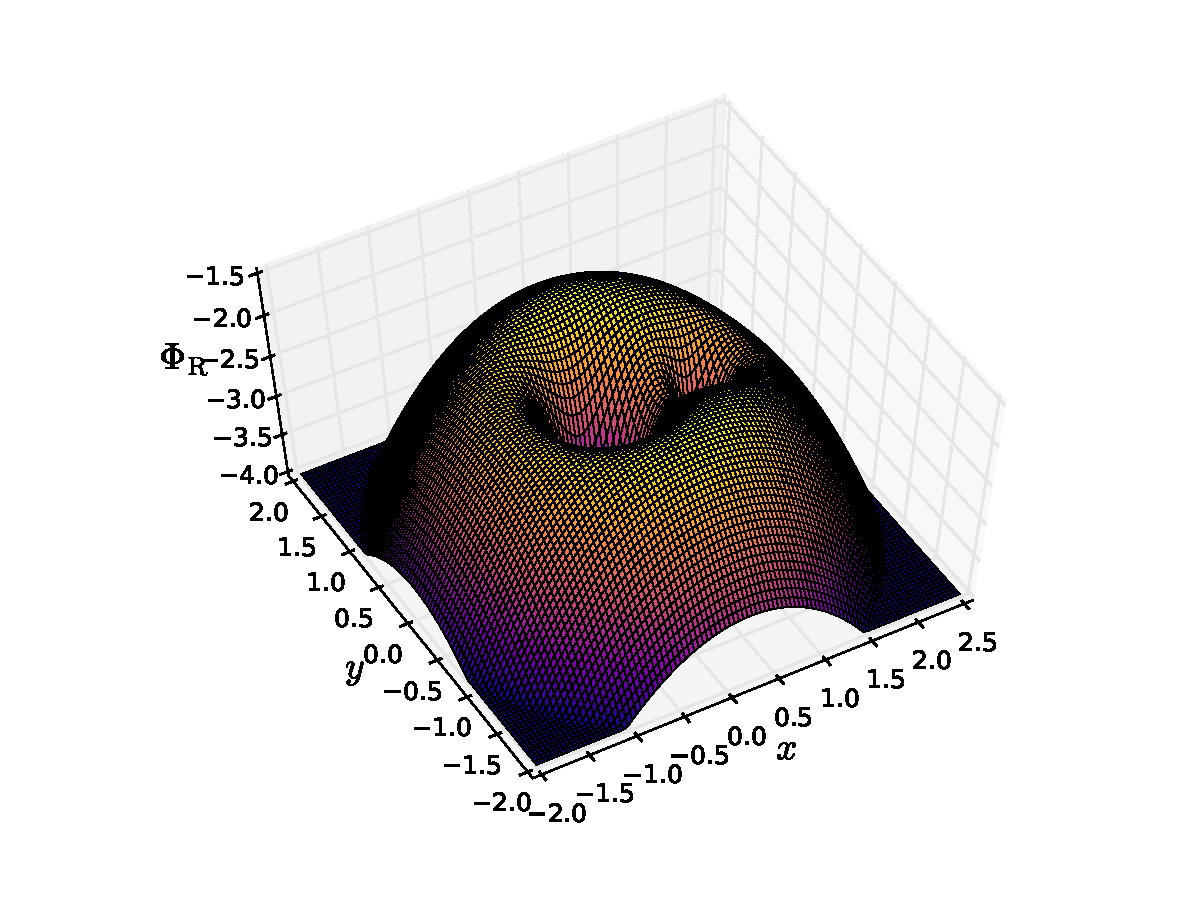
\includegraphics[width=7.5cm]{figs/astro/roche.pdf}
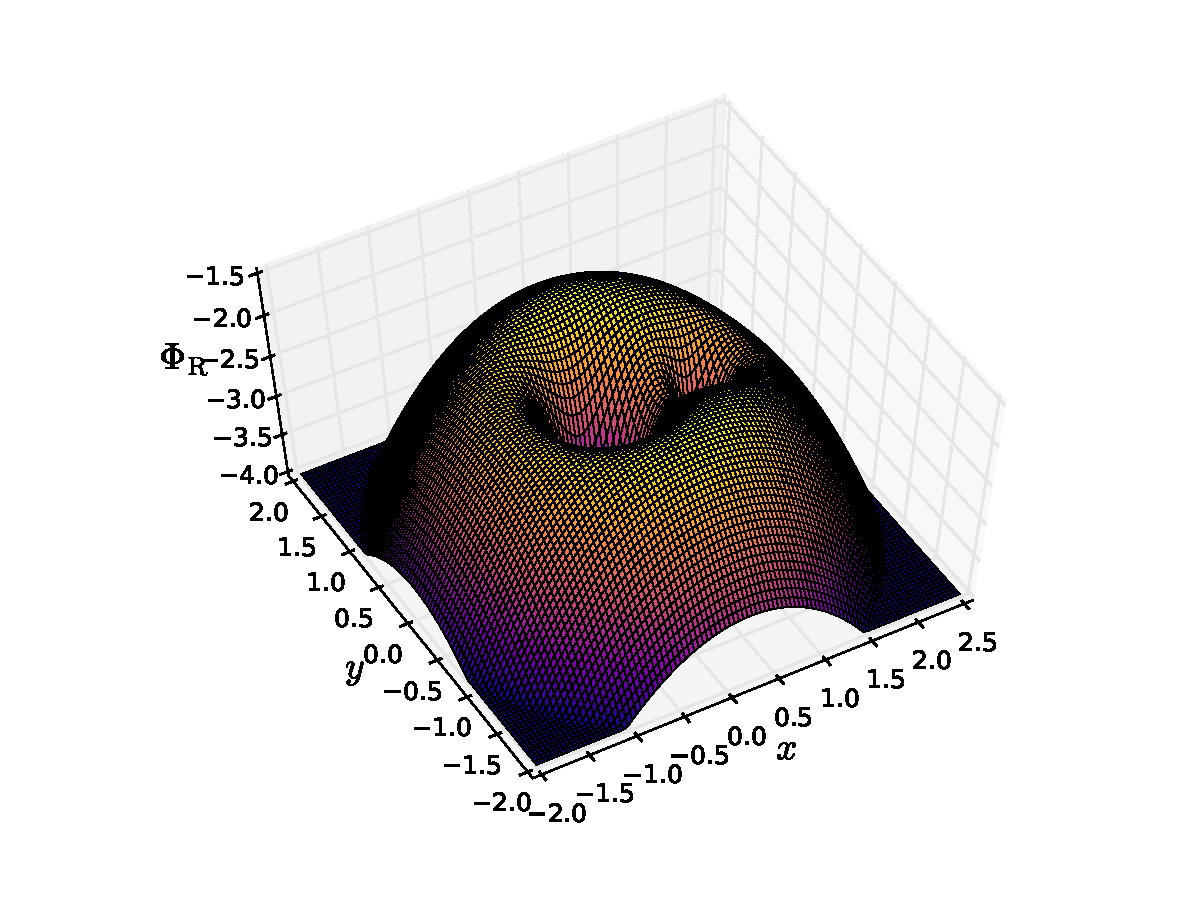
\includegraphics[width=7.5cm]{figs/astro/roche.pdf}
\caption{\label{fig:roche}
Roche potential for binary systems.
}
\end{figure}

\section{Accretion}
infalling matter leads to X-rays \cite{Lewin93}


\section{Roche lobe overflow}
Roche Lobe \cite{PRP02} \cite{LL15}

A flow of gas between two stars can be described by the Euler equation.
It gives the time evolution of the velocity $\vec{v}$ of the gas that has a pressure of $P$ and density $\rho$.
In a reference frame rotating together with the binary system with angular velocity $\omega$ the Euler equation takes the form 
\be
\frac{ \partial \vec{v} }{\partial t} + (\vec{v} \cdot \nabla)\vec{v} = -\nabla \Phi_{\mathrm{R}} - 2 \vec{ \omega } \times \vec{v} - \frac{1}{\rho} \nabla P,
\ee
where the angular velocity of the binary is then
\be
\vec{ \omega } = \left( \frac{ G M }{a^3} \right)^{1/2} \vec{e},
\ee
as given with the unit vector $\vec{e}$, normal to the orbital plane.
Here $M$ is the total mass of the system, i.e. $M = M_1 + M_2$, where $M_1$ and $M_2$ are the individual masses of the two stars in the system, respectively, and $a$ is their orbital separation.

The effects originating from the gravitation and from the centrifugal forces are encapsulated in the so-called Roche potential, given as a function of radial vector $\vec{r}$ as
\be
\Phi_{\mathrm{R}}(\vec{r}) = -\frac{G M_1}{|\vec{r} - \vec{r_1}|} -\frac{G M_2}{|\vec{r} - \vec{r_2}|} - \frac{1}{2} ( \vec{ \omega } \times \vec{v} )^2,
\ee
where the location of the stars is given with $\vec{r_1}$ and $\vec{r_2}$.

By studying the shape of the potential, we see that in between the stars, in the so-called $L_1$ point there exists a location where the individual gravitational pull from the stars is balanced.
This leads to a kinda of a nozzle in the system from which the material can leak from the less massive star to the more massive object.
Such a leaking, or a Roche lobe overflow, will then occur if the companion star's radius exceeds the size of its Roche lobe.
Typically such a thing can happen when the star evolves and expands at the end of its life cycle. 

LMXB \cite{TH06}


\section{Accretion disks}



Hard and soft state \cite{HvdK89}

alterate between these two states \cite{MDF14} \cite{DGK07}



